\subsection*{No-cloning theorem proof}
\begin{theorem}
There is no unitary operator $U$ on $\mathcal{H} \otimes H$ such that for all normalised states $|\psi\rangle_{A}$ and $|s\rangle_{B}$ in $H$
$$
U\left(|\psi\rangle_{A}|s\rangle_{B}\right)=e^{i \alpha(\psi, s)}|\psi\rangle_{A}|\psi\rangle_{B},
$$
for some real number $\alpha$ depending on $\psi$ and $s$.
\end{theorem}
\begin{proof}
Suppose we have two quantum systems $A$ and $B$.
We start from an unknown but pure quantum state in 
A, $|\psi\rangle_A$. This is the state which is going to be copied in $B$. We assume that the target slot starts out in some standard pure state, $|s\rangle$. Thus, the initial state is:
$$
|\psi\rangle \otimes|s\rangle .
$$
Then, we want an unitary time-evolution operator $U$ that effects the copying procedure, ideally,
$$
\ket{\psi}\otimes|s\rangle \stackrel{U}{\longrightarrow} U(|\psi\rangle \otimes|s\rangle)=e^{i\alpha_{\psi}}|\psi\rangle \otimes|\psi\rangle.
$$
It looks like that we actually performed the copying procedure for the state $\ket{\psi}$, however, this procedure has to work for any state and not only for a specific one. 
Suppose then, this copying procedure works for two particular pure states, $|\psi\rangle_A$ and $|\varphi\rangle_A$. Then we have
$$
\begin{array}{c}
U(|\psi\rangle \otimes|s\rangle)=e^{i\alpha_{\psi}}|\psi\rangle \otimes|\psi\rangle, \\
U(|\varphi\rangle \otimes|s\rangle)=e^{i\alpha_{\varphi}}|\varphi\rangle \otimes|\varphi\rangle
\end{array}.
$$
The inner product of these two equations gives
\begin{align*}
    \bra{s}\bra{\varphi}U^{\dagger}U|\psi\rangle|s\rangle &= e^{i(\alpha_{\psi} -\alpha_{\varphi})}(\bra{\varphi}\bra{\varphi})(\ket{\psi}\ket{\psi}),
    \\
    \langle\psi \mid \varphi\rangle&= e^{i(\alpha_{\psi} -\alpha_{\varphi})}(\langle\psi \mid \varphi\rangle)^{2}.
\end{align*}
We can then take the absolute value of the last expression, and the phase factor vanishes: 
\begin{equation*}
     |\langle \psi \mid \varphi\rangle|=|\langle\psi \mid \varphi\rangle|^{2}.
\end{equation*}
But, $x=x^{2}$ has only two solutions, $x=0$ and $x=1$, so either $|\psi\rangle=e^{i\gamma}|\varphi\rangle$ or $|\psi\rangle \perp |\varphi\rangle$. This means that we can theoretically clone only a precise state and its orthogonal states. However, this cannot be the case for two arbitrary states. Therefore, a single universal $U$ cannot clone a general quantum state. This proves the no-cloning theorem. 
\end{proof}


\subsection*{Quantum Teleportation}
In the teleportation protocol, the two parties (guess who)  share an entangled Bell State.  It is implemented via a CNOT gate between the state to be sent (suppose Alice is sending the state) and the part of entangled Bell state Alice has. The CNOT gate creates another entangled state whose measurement Alice will send to the second party, say it's Bob, to perform the measurements accordingly. So if you assume the state to be sent is 1 qubit state after CNOT you will have a 3 qubit state (as Bell sate is 2 qubit state). Now Alice will measure the middle qubit which will be the part of classical information she will communicate to Bob.

So, you see the controlled-NOT acts as an entangling operator without affecting the first qubit (here $\ket{\psi}$) and changing the entangled Bell state and hence its measurement outcome.
A general description of this cool phenomena is shown in figure: 
\begin{figure}[h!]
    \centering
    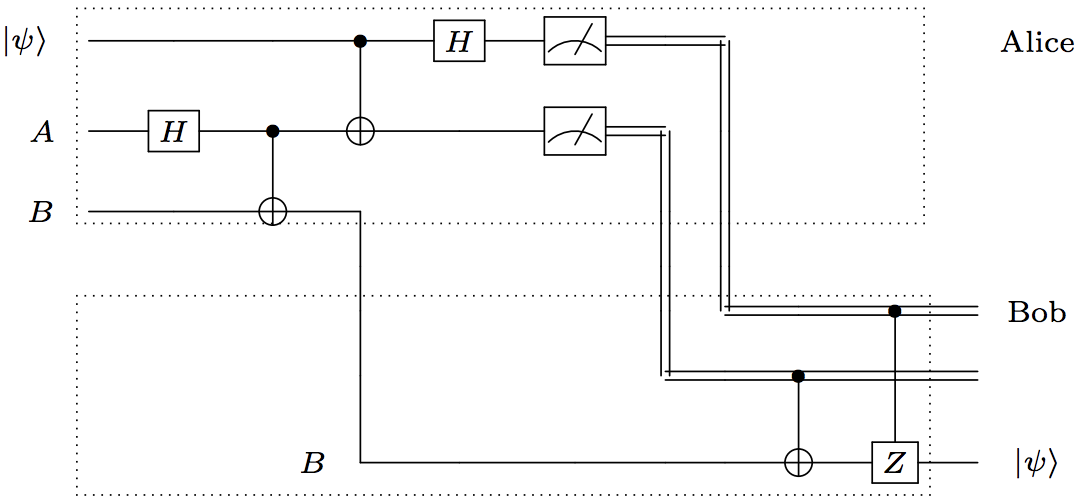
\includegraphics[width=\textwidth]{Mainmatter/images/teleportation-circuit.png}
    \caption{Basic circuit which implements quantum teleportation}
    \label{fig:teleportation}
\end{figure}
Quantum teleportation is very useful in quantum communication because it allows to send classical reliable bits instead of a qubit.